%\documentclass[11pt]{beamer}
%\usetheme{Montpellier}
%\usepackage[utf8]{inputenc}
%\usepackage{amsmath,mathtools}
%\usepackage{amsfonts}
%\usepackage{amssymb}
%\setbeamertemplate{footline}[frame number]
%%\setbeamercovered{transparent} 
%%\setbeamertemplate{navigation symbols}{} 
%%\logo{} 
%%\date{} 
%%\subject{} 



% !TEX TS-program = pdflatex
% !TEX encoding = UTF-8 Unicode

% This file is a template using the "beamer" package to create slides for a talk or presentation
% - Talk at a conference/colloquium.
% - Talk length is about 20min.
% - Style is ornate.

% MODIFIED by Jonathan Kew, 2008-07-06
% The header comments and encoding in this file were modified for inclusion with TeXworks.
% The content is otherwise unchanged from the original distributed with the beamer package.

\documentclass{beamer}




\definecolor {utorange}   {RGB} {203,96,21}
\definecolor {utblack}    {RGB} {99,102,106}
\definecolor {utbrown}    {RGB} {110,98,89}
\definecolor {utsecbrown} {RGB} {217,200,158}
\definecolor {utsecgreen} {RGB} {208,222,187}
\definecolor {utsecblue}  {RGB} {127,169,174}

\usepackage[orientation=landscape,size=custom,
	    width=16,height=9,scale=0.5,debug]{beamerposter}
%\usepackage{movie15}
\usepackage{graphicx}
\usepackage{amsmath}
%\usepackage{multimedia}
\usepackage[font={scriptsize,it}]{caption}
\usepackage[font={scriptsize,it}]{subcaption}
\usepackage[export]{adjustbox}
% Copyright 2004 by Till Tantau <tantau@users.sourceforge.net>.
%
% In principle, this file can be redistributed and/or modified under
% the terms of the GNU Public License, version 2.
%
% However, this file is supposed to be a template to be modified
% for your own needs. For this reason, if you use this file as a
% template and not specifically distribute it as part of a another
% package/program, I grant the extra permission to freely copy and
% modify this file as you see fit and even to delete this copyright
% notice. 


\mode<presentation>
{
  \usetheme{Boadilla}  
  \usefonttheme[onlymath] {serif}
  \setbeamercovered {invisible}
  \setbeamertemplate {navigation symbols} {}

  \setbeamercolor {normal text} {bg=white, fg=utblack}
  \setbeamercolor {structure} {fg=utorange}
  \setbeamercolor {alerted text} {fg=red!85!black}
  \setbeamercolor {item projected} {use=item,fg=black,bg=item.fg!35}
  \setbeamercolor* {palette primary} {use=structure,fg=white, bg=utorange}
  \setbeamercolor* {palette secondary} {use=structure,bg=utsecbrown}
  \setbeamercolor* {palette tertiary} {use=structure,bg=utsecgreen}
  \setbeamercolor* {palette quaternary} 
  		   {use=structure,fg=structure.fg,bg=utsecblue}
  \setbeamercolor* {framesubtitle} {fg=utbrown}
  \setbeamercolor* {block title} {parent=structure,fg=black,bg=utsecgreen}
  \setbeamercolor* {block body} {fg=black,bg=utblack!10}
  \setbeamercolor* {block title alerted} {parent=alerted text,bg=black!15}
  \setbeamercolor* {block title example} {parent=example text,bg=black!15}
\setbeamertemplate{itemize items}[circle]
\setbeamertemplate{enumerate items}[circle]
  \setbeamerfont {framesubtitle} {size=\small}
}

\DeclareMathOperator\supp{supp}
\newcommand{\red}[1]{{\color{red} #1}}
\newcommand{\blue}[1]{{\color{blue} #1}}
\newcommand{\green}[1]{{\color{green} #1}}
\newcommand{\black}[1]{{\color{black} #1}}
\newcommand{\cyan}[1]{{\color{cyan} #1}}
\newcommand{\chevron}[1]{\left\langle #1 \right\rangle}
\newcommand{\bigoh}[1]{\mathcal{O}\left( #1 \right)}
\newcommand{\pderiv}[2]{\frac{\partial #1}{\partial #2}}
\newcommand{\logdutauplus}{\pderiv{\log(u_{\tau})}{X^+}}
%\pgfdeclareimage [height=1.0cm] {utbig} {logos/UTWordmark}
%\pgfdeclareimage [height=0.6cm] {ut}    {logos/UTWordmark}
%
%\institute { \pgfuseimage {utbig}  }



%
%\addtobeamertemplate{frametitle}{}{
%  \begin{textblock*} {100mm} (0.95\textwidth, -0.75cm)
%     \pgfuseimage {ut}
%  \end{textblock*}
%}


\usepackage[english]{babel}
% or whatever

\usepackage[utf8]{inputenc}
% or whatever

\usepackage{times}
\usepackage[T1]{fontenc}
%\usepackage{tikz} % so that I can draw sherbs
\usepackage{pgfplots}
\pgfplotsset{compat=1.10}
\usepgfplotslibrary{fillbetween}
\usetikzlibrary{patterns}
\usetikzlibrary{tikzmark, decorations.pathreplacing}

% Or whatever. Note that the encoding and the font should match. If T1
% does not look nice, try deleting the line with the fontenc.


%\title[Thesis defense] % (optional, use only with long paper titles)
%{Numerical multiscale methods for boundary layer problems in fluid dynamics} % \\ $ \, $ \\ 
%\includegraphics[width =3.0 cm,height = 2.57 cm]{ICES_web_logo_2016.png}

%\author[Sean P. Carney] % (optional, use only with lots of authors)
%{Sean P. Carney}
%{Sean P. Carney \\ \footnotesize Joint work with Bj\"{o}rn Engquist and Robert D. Moser}
% - Give the names in the same order as the appear in the paper.
% - Use the \inst{?} command only if the authors have different
%   affiliation.

%\institute[The University of Texas at Austin] % (optional, but mostly needed)
%{
% %
%
%  Department of Mathematics \\
%  The University of Texas at Austin
%  }
% - Use the \inst command only if there are several affiliations.
% - Keep it simple, no one is interested in your street address.

%\date[May 2020] % (optional, should be abbreviation of conference name)
%{Committee members: Todd J. Arbogast, Bj\"{o}rn Engquist, Irene M. Gamba, Robert D. Moser, Yen-Hsi Richard Tsai }
%% - Either use conference name or its abbreviation.
%% - Not really informative to the audience, more for people (including
%%   yourself) who are reading the slides online

%\subject{LBNL 2019}
% This is only inserted into the PDF information catalog. Can be left
% out. 



% If you have a file called "university-logo-filename.xxx", where xxx
% is a graphic format that can be processed by latex or pdflatex,
% resp., then you can add a logo as follows:

 \pgfdeclareimage[height=0.5cm]{uni_primary}{uni_primary.jpg}
 \logo{\pgfuseimage{uni_primary}}
 \newcommand{\nologo}{\setbeamertemplate{logo}{}}



% Delete this, if you do not want the table of contents to pop up at
% the beginning of each subsection:
%\AtBeginSubsection[]
%{
%  \begin{frame}<beamer>{Outline}
%    \tableofcontents[currentsection,currentsubsection]
%  \end{frame}
%}

%%%%%%%%%%%%%%%%%%%%%%%%%%%%%%%%%%%%%%%%%
\newcommand{\R}{\mathbb{R}}
\newcommand{\N}{\mathbb{N}}
\newcommand{\Z}{\mathbb{Z}}
\newcommand{\Q}{\mathbb{Q}}
\newcommand{\C}{\mathbb{C}}
\newcommand{\Prj}{\mathbb{P}}
\newcommand{\F}{\mathbb{F}}
\newcommand{\A}{\mathbb{A}}
\newcommand{\Four}{\mathcal{F}}
\newcommand{\T}{\mathbb{T}}
\newcommand{\E}{\mathcal{E}}
\renewcommand{\L}{\mathcal{L}}
\newcommand{\eps}{\varepsilon}
%%%%%%%%%%%%%%%%%%%%%%%%%%%%%%%%%%%%%%%%%
\newcommand{\floor}[1]{\left\lfloor #1 \right\rfloor}
\newcommand{\ceil}[1]{\left\lceil #1 \right\rceil}
%\newcommand{\chevron}[1]{\langle #1 \rangle}
\newcommand{\norm}[1]{\left\lVert#1\right\rVert}
\newcommand{\paren}[1]{\left( #1 \right)}
\newcommand{\bracket}[1]{\left[ #1 \right]}
\newcommand{\abs}[1]{\left\lvert #1 \right\rvert}
%%%%%%%%%%%%%%%%%%%%%%%%%%%%%%%%%%%%%%%%%
\DeclareMathOperator{\id}{id}
\DeclareMathOperator{\convex}{conv}
\DeclareMathOperator{\image}{Im}
\DeclareMathOperator{\im}{Im}
\DeclareMathOperator{\coker}{coker}
%\DeclareMathOperator{\supp}{supp}
\DeclareMathOperator{\trace}{tr}
\DeclareMathOperator{\lspan}{span}
\DeclareMathOperator{\conv}{conv} % stands for conv, as in convex hull
\DeclareMathOperator{\Int}{int} % stands for int, as in interior of a set
\DeclareMathOperator{\sign}{sign}
\DeclareMathOperator{\ran}{ran}
\DeclareMathOperator{\rank}{rank}
%\DeclareMathOperator{\dim}{dim}
\newcommand{\dom}{\operatorname{dom}}
\newcommand{\cod}{\operatorname{cod}}
\newcommand{\Hom}{\operatorname{hom}}
\newcommand{\Ob}{\operatorname{Ob}}
\newcommand{\cl}{\operatorname{cl}}
\DeclareMathOperator{\BMO}{BMO}
%%%%%%%%%%%%%%%%%%%%%%%%%%%%%%%%%%%%%%%%%%
\newcommand{\del}{\partial}
\newcommand{\pvec}[2]{\frac{\partial #1}{\partial #2}}
\newcommand{\grad}{\nabla}
\newcommand{\ddt}{\frac{d}{dt}}
\renewcommand{\div}{\operatorname{div}}
\newcommand{\Laplace}{\Delta}
\newcommand{\kinet}{\bracket{\del_t + v\cdot \grad_x}}
\newcommand{\bessel}{\paren{1-\Laplace_v}}
\newcommand{\loc}{\text{loc}}
\newcommand{\Lip}{\text{Lip}}
%\newcommand{\BMO}{\text{BMO}}
\renewcommand{\Re}{\operatorname{Re}}
\newcommand{\ddz}{\frac{d}{dz}}
%%%%%%%%%%%%%%%%%%%%%%%%%%%%%%%%%%%%%%%%%%
\newcommand{\into}{\hookrightarrow}
\newcommand{\onto}{\twoheadrightarrow}
\newcommand{\isom}{\cong}
\newcommand{\rest}{{\upharpoonright}}
\newcommand{\weakly}{\rightharpoonup}
%%%%%%%%%%%%%%%%%%%%%%%%%%%%%%%%%%%%%%%%%%
\newcommand{\ith}{^\mathrm{th}}
\newcommand{\n}{^{-1}}
\newcommand{\half}{\frac{1}{2}}
%%%%%%%%%%%%%%%%%%%%%%%%%%%%%%%%%%%%%%%%%%
\newcommand{\indic}[1]{\chi_{\{#1\}}}
%%%%%%%%%%%%%%%%%%%%%%%%%%%%%%%%%%%%%%%%%%

%\author{Logan Stokols}
%\title{SQG on Bounded Domains}
%\subtitle{continuity at the boundary}
%\institute{UT Austin} 

\title[The De Giorgi Method: Applications]{The De Giorgi Method}
\subtitle{Applications to Degenerate PDE}

\author[Logan Stokols]
{ Logan F. Stokols}
%  {\small  The University of Texas at Austin}}

\institute[UT Austin] % (optional, but mostly needed)
{
 %

  Department of Mathematics \\
  The University of Texas at Austin
  }
%\institute[]{The University of Texas at Austin%Department of Mathematics,\\
%
%\newline
%\newline
%\newline
%\\
%}

\date[4 May 2020]{\footnotesize\em Thesis Defense, 4 May, 2020}
%\color{blue} {} \\[5pt]}
\begin{document}

\begin{frame}
\titlepage
\end{frame}

%-----------------------------------------------------

\begin{frame}{Outline}
\begin{enumerate}
\item Overview of the De Giorgi Method
\item Superquadratic Hamilton-Jacobi Equations
\item Hypoelliptic Fokker-Planck Equation
\item $L^2$-stability of Shocks
\item SQG on Bounded Domains
\end{enumerate}
\end{frame}

%-----%-----%-----%-----%-----%-----%-----%-----%-----%-----%-----%-----%
%-----%-----%-----% DG Method %-----%-----%-----%-----%-----%-----%-----%
%-----%-----%-----%-----%-----%-----%-----%-----%-----%-----%-----%-----%

\begin{frame}{Overview of De Giorgi Method}

Consider the toy problem
\[ \del_t u + \div(A\grad u) = 0 \]

\vskip.3cm
Given $\lambda I \leq A \leq \Lambda I$ (in sense of positive matrices), parabolic, expect regularity

\pause

\vskip.5cm
In fact, $\exists \alpha \in (0,1)$ s.t. $\forall \eps > 0$, $\exists C > 0$
\[ \norm{u}_{C^\alpha([\eps,\infty)\times \R^n)} \leq C \norm{u(0,\cdot)}_{L^2(\R^n)} \]
c.f. De Giorgi ['57]

\end{frame}

%-----------------------------------------------------

\begin{frame}{Energy Inequality}
Let $A \subseteq \R^n$, $[a,b]$ an interval, $\eps > 0$

\vskip.3cm

Multiply by test function $\phi(t,x) (u-k)_+$, obtain
\[ \sup_{[a,b]} \int_A (u-k)_+^2 + \int_a^b \int_A |\grad(u-k)_+|^2 \lesssim \int_{a-\eps}^b \int_{B_\eps(A)} (u-k)_+^2 \]

\end{frame}

%-----------------------------------------------------

\begin{frame}{First De Giorgi Lemma}
\begin{itemize}
\item $L^2$-to-$L^\infty$ regularization
\item global and local version
\item proof by truncation, recursion
\end{itemize}
\pause
\vskip.3cm
Consider $k \in \N$
\[ Q_0 := [-2,0]\times B_2 \supseteq Q_1 \supseteq \cdots \supseteq Q_k \supseteq \cdots \supseteq [-1,0]\times B_1 \]
%\[ [-1,0]\times B_1 \subseteq \cdots \subseteq Q_{k+1} \subseteq Q_k \subseteq \cdots \subseteq Q_0 := [-2,0]\times B_2 \]
and truncations
\[ u_0 := (u-0)_+ \geq u_1 \geq \cdots \geq u_k \geq \cdots \geq (u-1)_+ \]
%\[ (u-1)_+ \leq \cdots \leq u_{k+1} \leq u_k \leq \cdots \leq u_0 := (u-0)_+ \]

\end{frame}

%-----------------------------------------------------

\begin{frame}{First De Giorgi Lemma}
\begin{lemma}
Let $u$ solve parabolic equation, there exist $\delta_0$ small so
\[ \iint\limits_{Q_0} u_0^2 \leq \delta_0 \]
implies 
\[ \iint\limits_{[-1,0]\times B_1} (u-1)_+ = 0 \qquad \equiv \qquad u \leq 1 \textrm{ on } [-1,0]\times B_1 \]
\end{lemma}

\end{frame}

%-----------------------------------------------------

\begin{frame}{Proof of First De Giorgi Lemma}
Energy inequality says
\[ \underset{Q_k}{\sup \int} u_k^2 + \iint\limits_{Q_k} |\grad u_k|^2 \lesssim \iint\limits_{Q_{k-1}} u_k^2 \]
\pause
Sobolev embedding says, $\exists q > 2$
\[ \iint\limits_{Q_k} u_k^q \lesssim \paren{ \underset{Q_k}{\sup \int} u_k^2 + \iint\limits_{Q_k} |\grad u_k|^2 }^{q/2} \]
\pause
Basic Arithmetic says
\[ \iint\limits_{Q_k} u_k^2 \lesssim \iint\limits_{Q_k} u_{k-1}^q \]

\end{frame}

%-----------------------------------------------------

\begin{frame}{Proof of First De Giorgi Lemma}
Put together, 
\[ \iint\limits_{Q_{k+1}} u_{k+1}^2 \leq C_k \paren{ \iint\limits_{Q_k} u_k^2 }^{1+\eps} \]
if $u_0$ is sufficiently small on $Q_0$, then $(u-1)_+$ vanishes on $[-1,0]\times B_1$
\end{frame}

%-----------------------------------------------------

\begin{frame}{Second De Giorgi Lemma}
\begin{itemize}
\item also called Isoperimetric Inequality
\item quantitative version of ``solutions to parabolic eqn have no jump discontinuities''
\item can be non-constructive (compactness)
\item proof varies significantly between applications
\end{itemize}

\end{frame}

%-----------------------------------------------------

\begin{frame}{Second De Giorgi Lemma}
\begin{lemma}
$\exists \mu_0 > 0$ s.t., $u$ solving parabolic equation, if
\[ u \leq 2 \qquad \textrm{on } [-1,4]\times B_3, \]
\begin{align*} 
\textrm{and} && \abs{\{u \geq 1\} \cap [2,4]\times B_1} &\geq \delta_0, \\
\textrm{and} && \abs{\{u \leq 0\} \cap [0,4] \times B_2} &\geq \frac{1}{2} \abs{[0,4]\times B_2} \\
\textrm{then} && \abs{\{0<u<1\} \cap [0,4]\times B_2} &\geq \mu_0.
\end{align*}
\end{lemma}
\end{frame}

%-----------------------------------------------------

\begin{frame}{Proof of Second De Giorgi Lemma}
Assume false for all $\mu_0$, take sequence $u_k$ of counterexamples $\mu_0 = 1/k$
\vskip.3cm
By first condition and energy inequality, $u_k$ compact, has $L^2_t(H^1_x)$ limit $u_\infty$
\vskip.3cm
a.e. $t$ fixed, $\forall x$ either $u_\infty \geq 1$ or $u_\infty \leq 0$
\vskip.3cm
$u_\infty$ is $\leq 0$ on most of $[0,4]$ but $\geq 1$ on some of $[2,4]$, so energy increases suddenly in time, impossible

\end{frame}

%-----------------------------------------------------

\begin{frame}{H\"{o}lder Continuity}
Proof of H\"{o}lder continuity uses recursion
\vskip.3cm
apply two De Giorgi lemmas to rescalings of solution

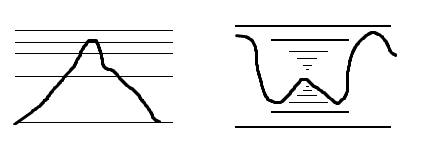
\includegraphics{Oscillation_and_Continuity}
\end{frame}

%-----%-----%-----%-----%-----%-----%-----%-----%-----%-----%-----%-----%
%-----%-----%-----% Hamilton-Jacobi %-----%-----%-----%-----%-----%-----%
%-----%-----%-----%-----%-----%-----%-----%-----%-----%-----%-----%-----%

\begin{frame}{Superquadratic Hamilton-Jacobi Equation}
\pause

\[\textrm{e.g.} \qquad \del_t u + |\grad u|^p - \eps \Laplace u = 0, \qquad \eps \in \{0,1,-1\} \]

\begin{itemize}
\item First considered by Lasry and Lions ('89), Schwab ('13) [homogenization]
\item Best known results Cardaliaguet ('09), Cannarsa and Cardaliaguet ('10), Cardaliaguet and Silvestre ('12)
\item $\eps = 0$ singularities can form, but solutions always continuous
\item For $p > 2$, continuous even for $\eps = -1$ [first order drives regularization]
\item Chan and Vasseur ('17) use De Giorgi for $\eps = 0$
\end{itemize}

\end{frame}

%-----------------------------------------------------

\begin{frame}{Superquadratic Hamilton-Jacobi Equation}
\[ \del_t u = H\paren{t,x,u,\grad u, D^2 u}, \]
\[ \Lambda\n |\grad u|^p - \div\paren{A \grad u} - f \leq H\paren{t,x,u,\grad u, D^2 u} \leq \Lambda |\grad u|^p - \Lambda m^-(D^2 u) + \Lambda \]
$p > 2$, $A$ bounded unsigned matrix, $f \in L^q$, $m^-$ returns lowest negative eigenvalue

\begin{theorem}[S., Vasseur [CMS, '18{]}]
Solutions (in appropriate weak sense) regularize from $L^\infty(\R^+\times\R^n)$ into $C^\alpha([\eps,\infty)\times \R^n)$
\end{theorem}
\end{frame}

%-----------------------------------------------------

\begin{frame}{Superquadratic Hamilton-Jacobi: Proof}
\begin{itemize}
\item De Giorgi method
\item Adapted technique of Chan, Vasseur, overcome second-order term
\item Combine divergence-form and non-divergence-form techniques
\item Allow unbounded source term $f$, discontinuous $A$
\end{itemize}
\end{frame}

%-----------------------------------------------------

\begin{frame}{Superquadratic Hamilton-Jacobi: Proof excerpt}
\pause
Consider
\[ \del_t u + \abs{\grad u}^p + \Laplace u = 0. \]
\pause
Using $\varphi(t,x) (u-k)_+$ as test function, obtain energy inequality
\[ \sup_{[-1,0]} \int_{B_1} (u-k)_+^2 + \int_{-1}^0 \int_{B_1} (u-k)_+ \abs{\grad (u-k)_+}^p \]
\[ \lesssim \int_{-2}^0 \int_{B_2} (u-k)_+^2 + \int_{-2}^0 \int_{B_2} \abs{\grad (u-k)_+}^2 \]
\pause
Want to show, on $Q_1 = [-1,0]\times B_1$, for some $q > 2$
\[ \norm{(u-1)_+}_{L^q(Q_1)} \lesssim \norm{(u)_+}_{L^\infty_t(L^2_x)(Q_1)} + \norm{(u)_+ |\grad (u)_+|^p}_{L^1(Q_1)}. \]
%\[ \int_{-1}^0 \int_{B_1} (u-1)_+^q \leq \paren{\sup_{[-1,0]} \int_{B_1} (u-k)_+^2 + \int_{-1}^0 \int_{B_1} (u-k)_+ \abs{\grad (u-k)_+}^p}^{1+\eps}. \]
%\[ \iint\limits_{Q_1} (u-1)_+^q \leq \paren{ {\sup \int}\limits_{Q_2} (u)_+^2 + \iint\limits_{Q_2}} \]

\end{frame}

%-----------------------------------------------------

\begin{frame}{Superquadratic Hamilton-Jacobi: Proof excerpt}
Coercivity when $u$ large
\vskip.3cm
\pause
Strategy: consider two regions, $u$ small and $u$ big \begin{itemize}
\item $u$ small $\Rightarrow$ $L^q$ norm small
\item $u$ big $\Rightarrow$ coercivity $\Rightarrow$ $L^q$ norm small
\end{itemize}
\pause
Implementation:
\begin{itemize}
\item $\norm{\grad (u-1)_+}_{L^p}^p \leq \norm{u_+ |\grad u_+|^p}_{L^1}$
\item $\norm{(u-1)_+}_{L^q} \lesssim \norm{(u-1)_+}_{L^\infty(L^2)} + \norm{\grad (u-1)_+}_{L^p}$
\end{itemize}
\end{frame}

%-----------------------------------------------------

%-----%-----%-----%-----%-----%-----%-----%-----%-----%-----%-----%-----%
%-----%-----%-----% Kinetic --%-----%-----%-----%-----%-----%-----%-----%
%-----%-----%-----%-----%-----%-----%-----%-----%-----%-----%-----%-----%

\begin{frame}{Hypoelliptic Fokker-Planck}
\pause
\[\textrm{e.g.} \qquad \bracket{\del_t + v\cdot\grad_x} f + \paren{-\Laplace_v}^s f = 0 \]

\begin{itemize}
\item Rarefied gas, neutral particles in plasma
\item Imbert and Silvestre ('16), Golse and Imbert and Mouhot and Vasseur ('16)
\item Hypoelliptic: non-elliptic regularization, mixed elliptic/hyperbolic type
\item Averaging Lemma (Golse et al '88): $H^s$ theory of hypoellipticity, regularity of averages for kinetic equation
\end{itemize}
\end{frame}

%-----------------------------------------------------

\begin{frame}{Hypoelliptic Fokker-Planck}
\[ \bracket{\del_t + v\cdot\grad_x} f = \int K [f(w)-f(v)] \,dw + \sigma \]
$K \approx |v-w|^{-(n+2s)}$, $s \in (0,1)$, $K$ symmetric in $(v,w)\mapsto(w,v)$ and in $(v,v+y)\mapsto(v,v-y)$

\begin{theorem}[S. [SIMA, '19{]}]
For $f$ solution, $f \in L^\infty \cap L^2_{t,x}(H^s_v)$, $\sigma \in L^2 \cap L^r$ for $r >> 1$, 
there exists $\alpha \in (0,1)$ depending on kernel, $C > 0$ depending on domain and kernel s.t.
\[ \norm{f}_{C^\alpha([\eps,\infty)\times\R^n\times B_1)} \leq C \paren{\norm{f}_{L^\infty} + \norm{\sigma}_{L^r}}. \]
\end{theorem}

\end{frame}

%-----------------------------------------------------

%\begin{frame}{Hypoelliptic Fokker-Planck: Proof}
%\begin{itemize}
%\item De Giorgi method 
%\item No distinction between $s \geq 1/2$, $s < 1/2$
%\item Averaging Lemma
%\end{itemize}
%
%\end{frame}

%-----------------------------------------------------

\begin{frame}{Hypoelliptic Fokker-Planck: Proof excerpt}
\pause
Consider $\Lambda = (-\Laplace_v)^{1/2}$, $s \in (0,1)$,
\[ \del_t f + v\cdot\grad_x f + \Lambda^{2s} f = 0. \]

Note diffusion in $v$ but not $x$!

Energy inequality will have
\[ \norm{(f-\psi)_+}_{L^\infty_t(L^2_{x,v})} + \norm{\Lambda^s (f-\psi)_+}_{L^2_{t,x,v}} \]
on LHS
\end{frame}

%-----------------------------------------------------

\begin{frame}{Averaging Lemma}
Lemma (B\'{e}zard, 94): for $\alpha = 1/(2(1+m))$, $\Omega \Subset \bar{\Omega} \subseteq \R^+ \times \R^n$, and $f,g \in L^2(\bar{\Omega} \times \R^n)$, $f$ compactly supported, we have
\[ \bracket{\del_t + v\cdot\grad_x} f = g \]
implies
\[ \norm{\int f \,dv}_{H^\alpha(\Omega)} \lesssim \norm{f}_{L^2(\bar{\Omega} \times \R^n)} + \norm{(1-\Laplace_v)^{-m/2} g }_{L^2(\bar{\Omega} \times \R^n)}. \]
\end{frame}

%-----------------------------------------------------

\begin{frame}{Hypoelliptic Fokker-Planck: Proof excerpt}
Unfortunately: Can't apply lemma to $(f-\psi)_+$ due to truncation (nonlocal)
\vskip.3cm

Barrier function
\[ 0 \leq \varphi(t,x) (f-\psi)_+ \leq F, \]
\[ \norm{F}_{L^2} + \norm{(1-\Laplace_v)^{-m/2} \bracket{\del_t + v\cdot\grad_x} F }_{L^2} \leq C \norm{\varphi (f-\psi)_+}_{L^2}. \]

\vskip.3cm

Now:
\[ \norm{\int F \,dv}_{H^\alpha} \leq \norm{\varphi (f-\psi)_+}_{L^2}, \]
No regularity on $f$!
%Using $\varphi(t,x)(f - \psi(v))_+$ as a test function, obtain
%\[ \sup_{[-1,0]} \int_{B_1} \int (f-\psi)_+^2 + \int_{-1}^0 \int_{B_1} \int \abs{\Lambda^s (f-\psi)_+}^2 \]\[ \lesssim \]

\end{frame}

%-----------------------------------------------------

\begin{frame}{Hypoelliptic Fokker-Planck: Proof excerpt}
From averaging lemma:
\[ \norm{(f-\psi)_+}_{L^{2+\eps}_{t,x}(L^1_v)} \lesssim \norm{(f-\psi)_+}_{L^2_{t,x,v}} \]
\pause
From energy inequality:
\[ \norm{(f-\psi)_+}_{L^\infty_t(L^2_{x,v})} + \norm{(f-\psi)_+}_{L^2_{t,x}(L^{2+\eps}_v)} \lesssim \norm{(f-\psi)_+}_{L^2_{t,x,v}} + \norm{(f-\psi)_+}_{L^1_{t,x,v}} \]
\pause
Improvement in all three variables, for some $q > 2$
\[ \norm{(f-\psi)}_{L^q_{t,x,v}} \lesssim \norm{(f-\psi)_+}_{L^2_{t,x,v}} \]
\pause
Control of regularity is means to an end, control of integrability is the end
\end{frame}

%-----%-----%-----%-----%-----%-----%-----%-----%-----%-----%-----%-----%
%-----%-----%-----% Stability of Shocks --%-----%-----%-----%-----%-----%
%-----%-----%-----%-----%-----%-----%-----%-----%-----%-----%-----%-----%

\begin{frame}{$L^2$ stability of Shocks}
\pause
Consider 1D scalar viscous conservation law
\[ \del_t u + \del_x[Q(u)] = \eps \del_{xx} \eta'(u) \]
where $\eta$, $Q$ uniformly elliptic and $\eps > 0$ arbitrary.

\begin{theorem}[S. [Submitted{]}]
For $u$ a solution and $s$ a sufficiently small shock solution, there exists Lipschitz $\gamma(t)$ such that
\[ \norm{u(\cdot,t) - s(\cdot-\gamma(t))}_2 \] 
stable in time, up to a constant factor.  Result is independent of $\eps$.  
\end{theorem}
\end{frame}

%-----%-----%-----%-----%-----%-----%-----%-----%-----%-----%-----%-----%
%-----%-----%-----% SQG %-----%-----%-----%-----%-----%-----%-----%-----%
%-----%-----%-----%-----%-----%-----%-----%-----%-----%-----%-----%-----%

\begin{frame}{SQG in Bounded Domains}
\pause
\[ \textrm{e.g.} \qquad \del_t \theta + \paren{\grad^\perp (-\Laplace)^{-1/2} \theta} \cdot \grad \theta + \nu (-\Laplace)^s \theta = 0 \]
\begin{itemize}
\item atmospheric or ocean currents, used in weather modelling
\item $\R^2$: Constantin, Majda, Tabak (93); Kiselev, Nazarov, Volberg (08); Caffarelli, Vasseur (10); Constantin, Vicol (12)
\item Bounded domain: Kriventsov ('15); Novack, Vasseur ('18,19)
\item Best studied model by Constantin, Ignatova ('16); Constantin, Ignatova, Nguyen (various)
\item Boundary issues: Laplacian \& gradient don't commute, Caffarelli-Stinga ('16) kernel representation degenerates
\end{itemize}
\end{frame}

%-----------------------------------------------------

\begin{frame}{SQG in Bounded Domains}
\begin{equation*}\begin{cases}
\del_t \theta + u \cdot \grad \theta + \Lambda \theta = 0, \\
u = \grad^\perp \Lambda^{-1} \theta.
\end{cases} \end{equation*}
$\Omega \subseteq \R^2$ smooth bounded open, $\Lambda := \sqrt{-\Laplace_D}$ (defined spectrally), $\Laplace_D$ the Dirichlet Laplacian on $\Omega$

\begin{theorem}[S., Vasseur [ARMA, '20{]}]
Let $\Omega \subseteq \R^2$ a bounded set, initial data $\theta_0 \in L^2(\Omega)$

There exists a global-in-time solution $\theta$ to SQG such that:

For any $\eps > 0$, there exists $\alpha \in (0,1)$ and a constant $C$ so
\[ \norm{\theta}_{C^\alpha([\eps,\infty)\times\Omega)} \leq C \norm{\theta_0}_{L^2(\Omega)}. \]
\end{theorem}

\end{frame}

%-----------------------------------------------------

%\begin{frame}{SQG in Bounded Domains: Proof}
%\begin{itemize}
%\item De Giorgi method, Caffarelli, Vasseur (2010)
%\item Boundary issues: Laplacian \& gradient don't commute, Caffarelli-Stinga ('16) kernel representation degenerates
%\end{itemize}
%
%\end{frame}

%-----------------------------------------------------

\begin{frame}{SQG in Bounded Domains: Proof excerpt}
\pause
Velocity $u$, energy inequality with cutoff $\Psi$ has drift term on RHS
\[ \int_\Omega u (\theta-\Psi)_+ \cdot \textrm{d}\Psi \]

recall $u$ is Riesz transform of $\theta \in L^\infty$

\begin{table}
\begin{tabular}{l | c | c | c }
$u$ bounded in: & $L^\infty$ & BMO & $B^0_{\infty,\infty}$ \\
\hline \hline
$\theta \in L^\infty \Rightarrow u \in \underline{\quad}$ & $\times$ & works on $\R^2$ & complicated \\[.3cm]
$\int u \theta_+$ bounded & $\leq \int \theta_+$ & John-Nirenberg & complicated \\[.3cm]
scaling invariant & \checkmark & \checkmark & \checkmark
\end{tabular}

\end{table}

%\vskip .5cm
%
%\begin{equation*}
%* = \begin{cases}
%u_\ell = \sum_{j=-\infty}^0 \Delta_j u, \qquad u_h = \sum_{j=0}^\infty \Delta_j u \\
%\int u_\ell \theta_+ + \int u_h \theta_+ \leq \int \theta_+ + \int |\Lambda^\eps \theta_+|
%\end{cases}
%\end{equation*}



\end{frame}

%-----------------------------------------------------

\begin{frame}{Control on u: Littlewood Paley theory}
Littlewood paley operators $P_j=P_j(\Lambda)$, functional calculus for $\Lambda$,
\vskip.3cm
Bernstein Inequalities
\begin{align*} 
\norm{\Lambda^s P_j f}_p &\approx 2^{sj} \norm{f}_p, \\
\norm{\grad \Lambda P_j f}_p &\approx 2^{(1+s)j} \norm{f}_p.
\end{align*}
Commutation Relation
\[ \norm{P_i \grad P_j f}_p \lesssim \min(2^j,2^i) \norm{f}_p. \]

\vskip.5cm

Bernstein: Iwabuchi, Matsuyama, Taniguchi (``Bilinear estimates in Besov spaces generated by the Dirichlet Laplacian'' 2017)
\end{frame}

%-----------------------------------------------------

\begin{frame}{Control on u: high and low frequencies}

Instead of Besov norm $\sup_j \norm{P_j \grad \Lambda\n \theta}_\infty$ consider
\[ \grad \Lambda\n P_j \theta. \]

To bound $\int u \theta_+$, decompose as
\[ u_{\textrm{low}} = \sum_{j=-\infty}^0 \grad \Lambda\n P_j \theta \]
which is Lipschitz,
\[ u_{\textrm{high}} = \sum_{j=0}^\infty \grad \Lambda\n P_j \theta \]
which is in $W^{-\eps, \infty}$.  

\end{frame}

%-----------------------------------------------------

%-----------------------------------------------------

%-----------------------------------------------------

\begin{frame}
\centering \Large
Thank you

\end{frame}


\end{document}